\documentclass[aspectratio=169]{beamer}

% Default packages
\usepackage[T1]{fontenc}
\usepackage[english]{babel}
\usepackage{pgfplots}
\pgfplotsset{compat=newest}
\usepackage{booktabs}
\usepackage{siunitx}
\usepackage{amsmath}

% Font selection
% Latin Modern
\usepackage{lmodern}
% Verdana font type
%\usepackage{verdana}
% Helvetica
%\usepackage{helvet}
% Times (text and math)
%\usepackage{newtx, newtxmath}
% Nice font combination
%\usepackage{mathptmx} % math
%\usepackage{sourcesanspro} % sans-serif
\usepackage{charter} % serif

%Avoid shaded in RMarkdown



% Use DTU theme, see below for options
\usetheme[department=compute]{DTU}

\title[Automated and Early Detection of Disease Outbreaks]{Farrington
and Noufaily}
\author{Kasper Schou Telkamp}
\institute{Section for Dynamical Systems}
\date{2023-03-02}
	
\newcommand{\tabitem}{{\color{dtured}$\bullet$} }

\DeclareMathOperator{\E}{E}
\DeclareMathOperator{\G}{G}
\DeclareMathOperator{\N}{N}
\DeclareMathOperator{\NB}{NB}
\DeclareMathOperator{\Pois}{Pois}
\DeclareMathOperator{\Geom}{Geom}


\begin{document}


\frame{
	\maketitle
}

\frame{
	\frametitle{Outline}
	\tableofcontents
}

\hypertarget{data-exploration}{%
\section{Data exploration}\label{data-exploration}}

\hypertarget{vtec-stec}{%
\subsection*{VTEC / STEC}\label{vtec-stec}}

\begin{frame}{VTEC / STEC}
\tiny

\begin{table}
\centering\begingroup\fontsize{12}{14}\selectfont

\begin{tabular}{llll}
\toprule
Date & ageGroup & y & n\\
\midrule
2008-01-01 & <1 year & 2 & 64137\\
2008-01-01 & 1-4 years & 2 & 259910\\
2008-01-01 & 5-14 years & 2 & 680529\\
2008-01-01 & 15-24 years & 1 & 631724\\
... & ... & ... & ...\\
2022-12-01 & 55-64 years & 2 & 773073\\
2022-12-01 & 65-74 years & 5 & 621965\\
2022-12-01 & 75-84 years & 4 & 449423\\
2022-12-01 & 85+ years & 3 & 132181\\
\bottomrule
\end{tabular}
\endgroup{}
\end{table}

\normalsize
\end{frame}

\hypertarget{vtec-stec-1}{%
\subsection{VTEC / STEC}\label{vtec-stec-1}}

\begin{frame}{VTEC / STEC}
\tiny

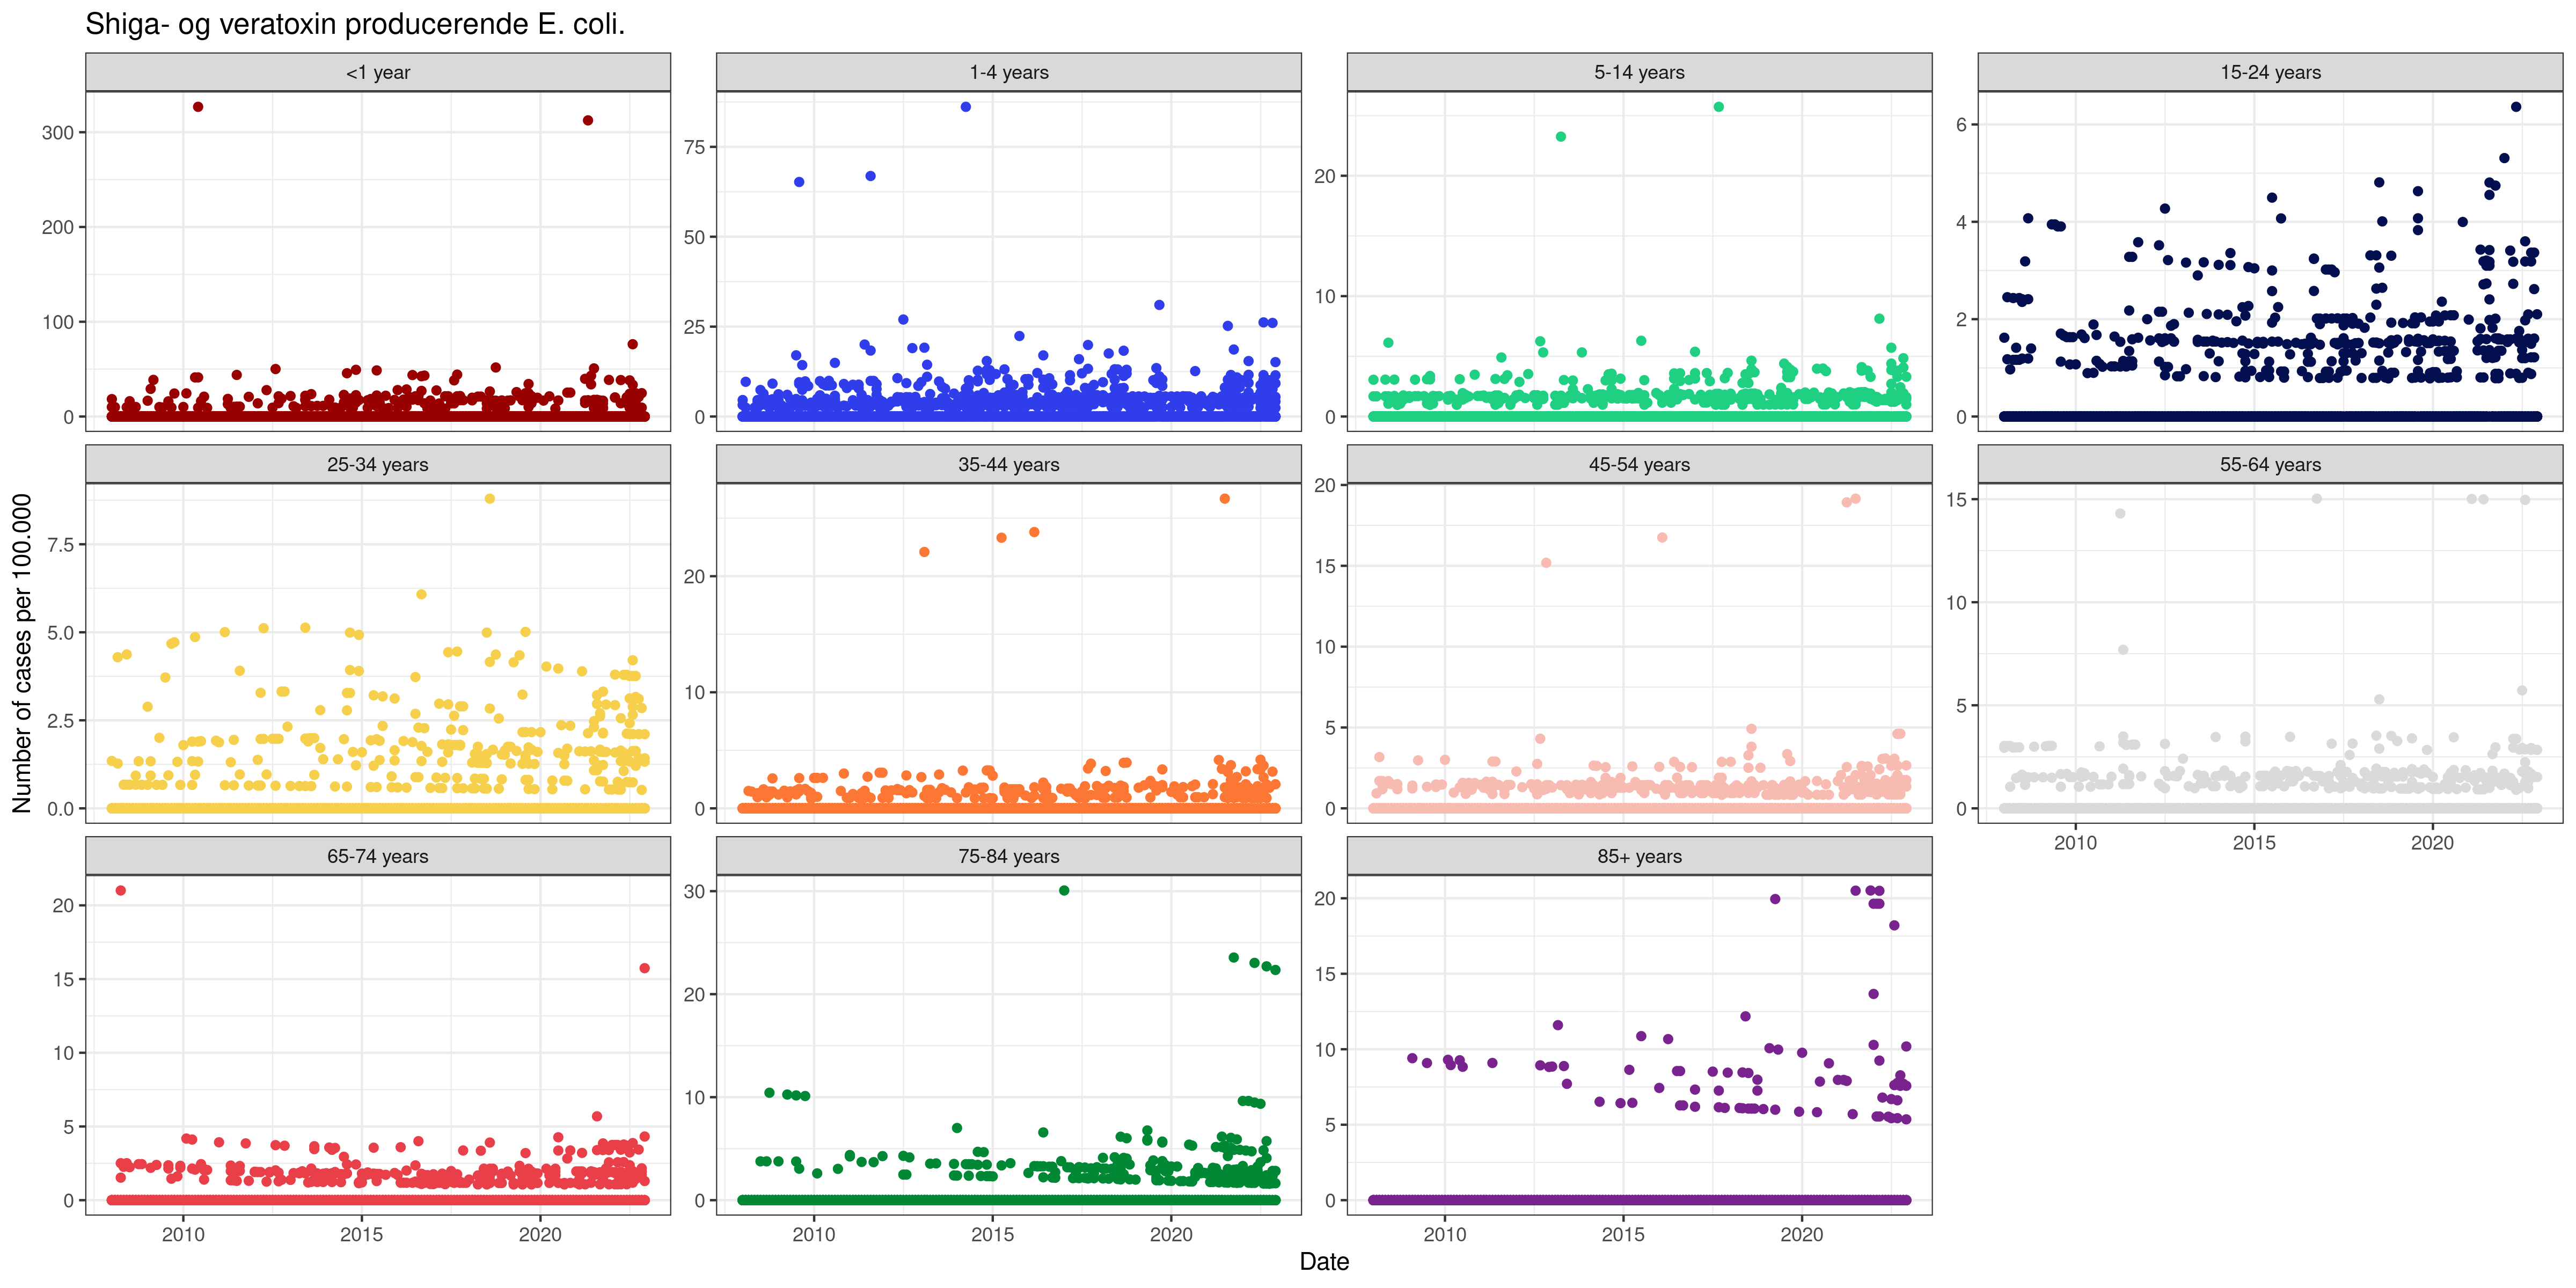
\includegraphics[width=1\linewidth]{../figures/ShigaogveratoxinproducerendeEcolixAgeGroup}

\normalsize
\end{frame}


\end{document}
